\documentclass[10pt,letterpaper]{article} 
\usepackage{toolsper}
%\usepackage{graphicx}‎‎
%\usefonttheme{serif}‎
%\usepackage{ptext}‎
\usepackage{xepersian}
\settextfont{B Nazanin}
\usepackage{lipsum}
\setlength{\parindent}{0pt}
\newcommand{\pf}{$\blacksquare$}
\newcommand{\pic}[2]{
\begin{center}
\includegraphics[width=#2]{#1}
\end{center}
}
\begin{document}
\Large
\begin{center}
به نام خدا

پاسخ تمرینات سری دوم درس آمار و احتمال
\hl
\end{center}
سوالات 13، 22 ، 24 و 25 از کتاب غیرمرجع (کتاب 
\lr{
Probability, Random Variables and Stochastic Processes
}
 از پاپولیس
)
\np
{\color{red}
سوالات 13 و 25 از کتاب غیرمرجع، به دلیل کاربرد متغیرهای تصادفی سوالات امتیازی محسوب می‌شوند.
}
\np
سوال 13) تعریف کنید
$$
f(t_0)\triangleq P\{t\ge t_0\}
$$
در اینصورت باید نشان دهیم
$$
P\Big([t_0\le t\le t_0+t_1] \cap [t\ge t_0]\Big)=f(t_0)\Big[1-f(t_1)\Big]
$$
یا به عبارت دیگر
$$
P(t\ge t_0)-P(t\ge t_0+t_1)=f(t_0)-f(t_0)f(t_1)
$$
طبق تعریف
$$
f(t_0)-f(t_0+t_1)=f(t_0)-f(t_0)f(t_1)
$$
یا معادلا
$$
f(t_0+t_1)=f(t_0)f(t_1)
$$
می‌توان ثابت کرد تنها تابع پیوسته ای که شرط بالا را برآورده می‌کند‌، تابع نمایی است بنابراین 
$
f(t_0)=e^{-ct_0}
$
 که $c>0$ و اثبات کامل است $\blacksquare$
\np
سوال 22) می دانیم که برای استقلال رخدادهای 
$
A_1,A_2,\cdots ,A_n
$
 باید هر ترکیب چندتایی از این رخدادها مستقل باشند؛ یعنی هر دوتایی از آنها، هر سه تایی از آنها، ... و همه‌ی $n$ تا از آنها. چون دقیقا 
$
\binom{n}{k}
$
 ترکیب $k$ تایی از این مجموعه ها وجود دارد، در اینصورت باید دقیقا
$$
\sum_{k=2}^{n}\binom{n}{k}=2^n-n-1
$$
 معادله داشته باشیم.
\np
سوال 24) (در این مسئله بهتر است خرابی هر دو لامپ را یک پیشامد در نظر بگیریم؛ زیرا تنها این پیشامد به همراه پیشامد انتخاب جعبه مورد سوال است. هر چند مسئله را می توان از طریق تعریف یک پیشامد برای هر لامپ نیز حل کرد. این هنر فرد است که پیشامدها و رخدادها را به صورت \textbf{کاملا درست و واضح} و البته تا حد امکان \textbf{حداقلی} تعریف کند تا دقیقا همان مسئله ای را حل کند که از او خواسته شده و البته همان مسئله را هم به صورت خلاصه و حداقلی حل نماید. تناقض برتراند، نمونه‌ی بسیار خوبی از حل مسئله‌ی احتمالی به چند روش ممکن فقط بر اساس تخصیص احتمال های مختلف به رخدادهاست.)

 الف)
$$
A=\{\text{\rl{
پیشامد خرابی هر دو لامپ
}}\}
$$
$$
B=\{\text{\rl{
پیشامد انتخاب جعبه‌ی 1
}}\}
$$
در این سوال داریم
$$
P(A|B)={\binom{100}{2}\over\binom{1000}{2}}\approx 0.01
$$
$$
P(A|B^c)={\binom{100}{2}\over\binom{2000}{2}}\approx 0.0025
$$
$$
P(B)={1\over 2}
$$
و مطلوب ما 
$
P(A)
$
 است؛ در اینصورت طبق قاعده‌ی احتمال کل
\eqn{
P(A)
&=P(B)P(A|B)+P(B^c)P(A|B^c)
\\&=
{1\over 2}(0.01+0.0025)
\\&=0.0063
}{}
ب) مطلوب ما 
$
P(B|A)
$
 است. در اینصورت
\eqn{
P(B|A)&={P(AB)\over P(A)}
\\&={P(B)P(A|B)\over P(A)}
\\&={0.5\times 0.01\over 0.0063}
\\&=0.7937
}{}
این احتمال، احتمال قابل توجهی است زیرا درصد تعداد لامپ‌های خراب در جعبه‌ی 1 بیشتر است.
\np
سوال 25) اگر $X$ و $Y$ را به ترتیب متغیرهای تصادفی ورود قطار و اتوبوس به ایستگاه بدانیم، این متغیرها دارای توزیع یکنواخت بین ساعتهای 9 و 10 و مستقل هستند. در اینصورت قطار بازه‌ی زمانی 
$
\left(X,X+{1\over 6}\right)
$
 و اتوبوس بازه‌ی زمانی 
$
\left(Y,Y+x\right)
$
 را اشغال می کند. مکمل این پیشامد، حالتی است که اتوبوس و قطار یکدیگر را ملاقات نکنند؛ یعنی
$$
Y>X+{1\over 6}
\qquad
\text{\rl{
 یا 
}}
\qquad
Y+x<X
$$
 در اینصورت پیشامد مطلوب ما خواهد بود:
$$
X-x<Y<X+{1\over 6}
$$
که مساحت ناحیه‌ی زیر است:
\begin{center}
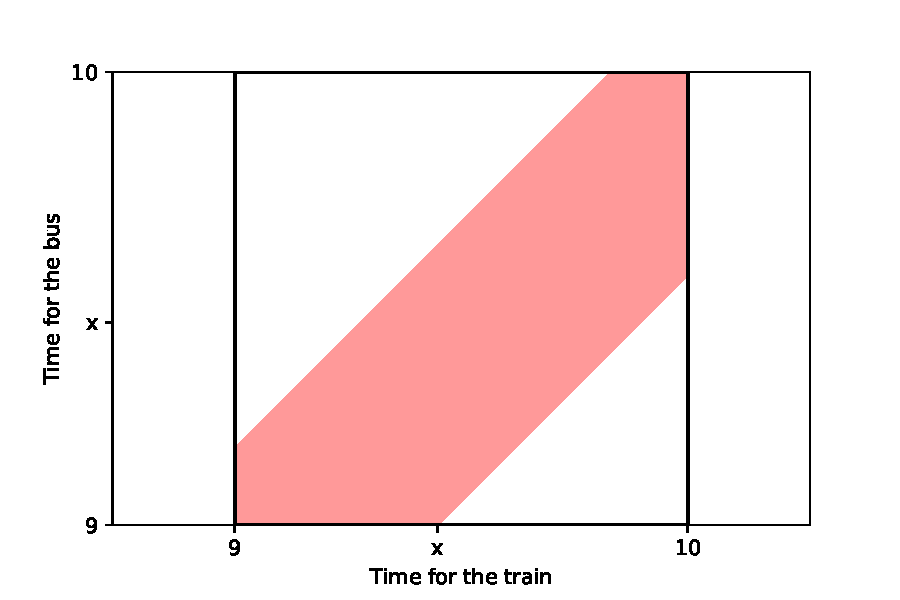
\includegraphics{HW2_Q.pdf}
\end{center}
مساحت ناحیه‌ی هاشور نخورده برابر است با
$$
{25\over 72}+{(1-x)^2\over2}
$$
این مساحت باید برابر $1\over 2$ باشد که در این‌صورت مقدار $x$ برابر 
$
1-{\sqrt{11}\over 6}\approx0.4472 \text{\lr{h}}\approx \text{\rl{27 دقیقه}}
$
 محاسبه می شود.
\np
سوالات 13، 22 و 24 از کتاب مرجع (کتاب 
\lr{
Probability and Statistics
}
 از پاپولیس
)
\np
سوال 13) این مسئله به کمک قانون احتمال کل و استفاده از تعریف احتمال شرطی به راحتی قابل حل است \pf
\np
سوال 22) مشابه سوال 22 از کتاب غیر مرجع.
\np
سوال 24) رشته‌ی لامپ زمانی کار می‌کند که تمام لامپ های آن سالم باشند (تقسیم ولتاژ و خاصیت سری بودن؛ در حالت موازی، کافی است حداقل یکی از لامپ ها کار کند به دلیل تقسیم جریان) در اینصورت خواهیم داشت:
\eqn{
p=(1-0.01)^{50}\approx 0.61
}{}
\np
\textbf{
\rl{
سوالات تالیفی
}
}

سوال 1) 
\eqn{
&
P(F)=0.37
\\&
P(M)=0.43
\\&
P(D|M)=0.15
\\&
P(D|F)=0.25
}{}
مطلوب است 
$
P(D|M\cup F)
$.
 در اینصورت داریم
\eqn{
P(D|M\cup F)&=
{P(D\cap[M\cup F])\over P(M\cup F)}
\\&=
{P([D\cap M]\cup [D\cap F])\over P(M)+P(F)}
\\&=
{P(D\cap M)+P(D\cap F)\over P(M)+P(F)}
\\&=
{P(M)P(D|M)+P(F)P(D|F)\over P(M)+P(F)}
\\&=
{0.37\times 0.25+0.43\times 0.15\over 0.8}
\\&\approx 0.20
}{}
این مسئله را به گونه‌ی دیگری نیز می توان حل کرد. از آنجا که به طور کل کودکان در سوال مطرح نمی‌شوند نسبت جمعیت زنان و مردان بزرگسال را به کل بزرگسالان محاسبه می کنیم. به طور کل، 
$
53.75\%
$
 جمعیت بزرگسالان را مردان و
$
46.25\%
$
 را زنان تشکیل می دهند. بنابراین می توان نوشت
\eqn{
&
P(M)=0.5375
\\&
P(F)=0.4625
}{}
و مطلوب 
$
P(D)
$
 خواهد بود؛ در این صورت
\eqn{
P(D)&=
P(D\cap M)+P(D\cap F)
\\&=
P(D|M)P(M)+P(D|F)P(F)
\\&=
0.5375\times 0.15+0.4625\times 0.25
\\&\approx 0.20
}{}
\np
سوال 2)
\eqn{
P(A|B\cap C)&=
{P([A\cap B]\cap [A\cap C])\over P(B)P(C)}
}{}
برای آنکه تساوی ارضا شود، یک شرط کافی مستقل بودن $A\cap B$ و $A\cap C$ است.
\np
سوال 3) کران بالا به وضوح بنا به رابطه‌ی احتمال اجتماع برقرار است. این کران بسیار مهم، \textbf{\rl{کران اجتماع}}
\footnote{
\lr{Union Bound}
}
 نامیده می شود.

برای اثبات کران پایین، ابتدا به دلیل تقارن فرض می کنیم 
$
P(A)\le P(B)
$
. اکنون کافی است مد نظر قرار دهیم که نامساوی های زیر معادلند:
\eqn{
&
P(A)+P(B)-{1\over 4-4P(A)}\le P(A\cup B)
\\& \iff
{1\over 4-4P(A)}\ge P(A\cap B)
\\& \iff
P(A\cap B)(1-P(A))\le {1\over 4}
}{}
از آنجایی که $
P(A\cap B)\le P(A)
$
 و بیشینه مقدار $u-u^2$ به ازای $0<u<1$ در $u={1\over 2}$ رخ می‌دهد، اثبات کامل است \pf
\end{document}